\documentclass[12pt, titlepage]{article}
\usepackage{graphicx}
\usepackage{float}
\restylefloat{table}

% Imported Packages
%------------------------------------------------------------------------------
\usepackage{amssymb}
\usepackage{amstext}
\usepackage{amsthm}
\usepackage{amsmath}
\usepackage{enumerate}
\usepackage{fancyhdr}
\usepackage[margin=1in]{geometry}
\usepackage{graphicx}
\usepackage{extarrows}
\usepackage{setspace}
%------------------------------------------------------------------------------

% Header and Footer
%------------------------------------------------------------------------------
\pagestyle{plain}  
\renewcommand\headrulewidth{0.4pt}                                      
\renewcommand\footrulewidth{0.4pt}       
\newcommand\tab[1][1cm]{\hspace*{#1}}                                 
%------------------------------------------------------------------------------

% Title Details
%------------------------------------------------------------------------------
\title{SE 3A04: Software Design III: Large System Design}
\author{Group \#5, Spaceship System Sabotage %Alliteration; always adored and absolutely amazing
		\\Pareek Ravi 001407109
		\\Pavle Arezina 001410366
		\\David Hobson 001412317
		\\Victoria Graff 001401451
		\\Julian Cassano 001406891
}
\date{\today}                          
%------------------------------------------------------------------------------

% Document
%------------------------------------------------------------------------------
\begin{document}

\maketitle	
\pagenumbering{arabic}
\tableofcontents
\listoftables
\listoffigures
\newpage

\section{Introduction}
\label{sec:introduction}
% Begin Section

\subsection{Purpose}
\label{sub:purpose}
% Begin SubSection
\tab The purpose of this document is to break down of the interactions and structure of the classes within the system into their separate objects. The document utilizes high level design by taking previously analysis on how the system will be utilized and developing the classes and objects that will be utilized to form the system. Interaction and behaviour of objects are designed to conform to the thorough analysis conducted to achieve the requirements of the system.  The intended audience for this document is for the developers implementing the system, technical guidelines for quality assurance analysts and developers to maintain the system, and stakeholders who have knowledge of software design who would like a more detailed overview of the system.
% End SubSection

\subsection{System Description}
\label{sub:system_description}
\tab Space system sabotage is a simulation of a fictional spaceship that is travelling to a pre-determined location in a fixed amount of time. The user will interact with the system through random events based on a function of the running time of the simulation. Random events will involve negative situations that occur, such as comets damaging the ship or part of the ship being sabotaged, where the user will have to respond to fix them in a timely manner with a selection of tools. If successful, the space ship continues toward its goal but if an incorrect solution was chosen then the problem is spread to other systems. If enough events happen with incorrect solutions to them, then the space ship will slowly spiral out of control and the user will fail the simulation. This system offers an entertaining environment to the user where they will be challenged to keep the spaceship intact until it dock import at the space station.

\subsection{Overview}
\label{sub:overview}
% Begin SubSection
\tab The rest of this document is separated into three sections, the first being the state charts for controller classes. These diagrams describe the dynamic behaviour of a system in response to external stimuli. They are especially useful in modelling reactive objects whose states are triggered by specific events. The next section entails the sequence diagrams of the system. Interactions between among classes in terms of exchange of messages over time are documented in the sequence diagrams. There is usually one for each use case found for the system. The last section is composed of the class diagram that describes the static structure of the system. Class diagrams are the backbone of almost every object orientated method, such as the UML method utilized for this document. After these three sections, there is the appendix that includes the division of labour. 

% End SubSection

% End Section

\section{State Charts for Controller Classes}
\label{sec:state_charts_for_controller_classes}

% Begin Section
\subsection*{Tool Controller}
\begin{figure}[H]
\centering
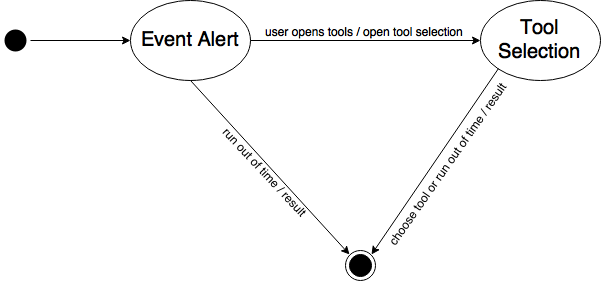
\includegraphics[width=120mm]{ToolController.png}
\caption{Tool Controller State Chart}
\end{figure}

\subsection*{Control Object}
\begin{figure}[H]
\centering
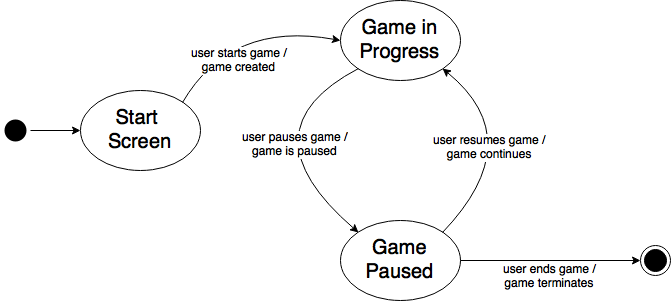
\includegraphics[width=120mm]{ControlObject.png}
\caption{Tool Controller State Chart}
\end{figure}

\subsection*{Power Controller}
\begin{figure}[H]
\centering
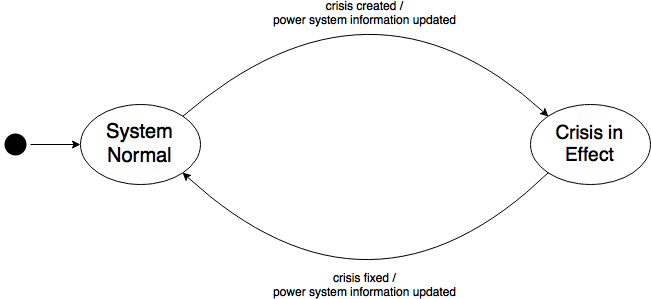
\includegraphics[width=120mm]{PowerController.png}
\caption{Power Controller State Chart}
\end{figure}

\subsection*{Mechanical Controller}
\begin{figure}[H]
\centering
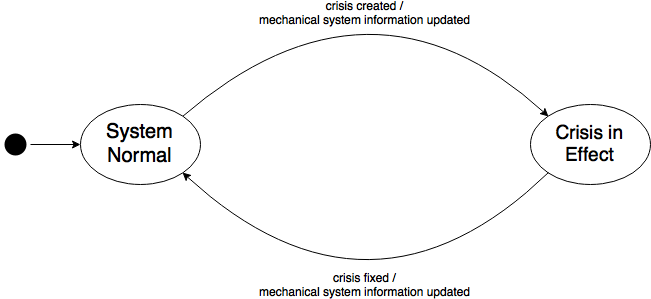
\includegraphics[width=120mm]{MechanicalController.png}
\caption{Mechanical Controller State Chart}
\end{figure}

\subsection*{Oxygen Controller}\begin{figure}[H]
\centering
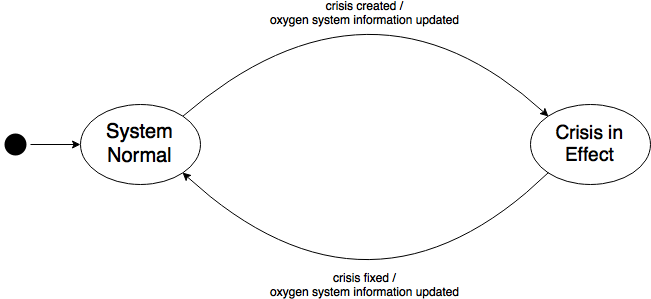
\includegraphics[width=120mm]{OxygenController.png}
\caption{Oxygen Controller State Chart}
\end{figure}

\subsection*{Overall Controller}
\newpage
\begin{figure}[H]

\centering
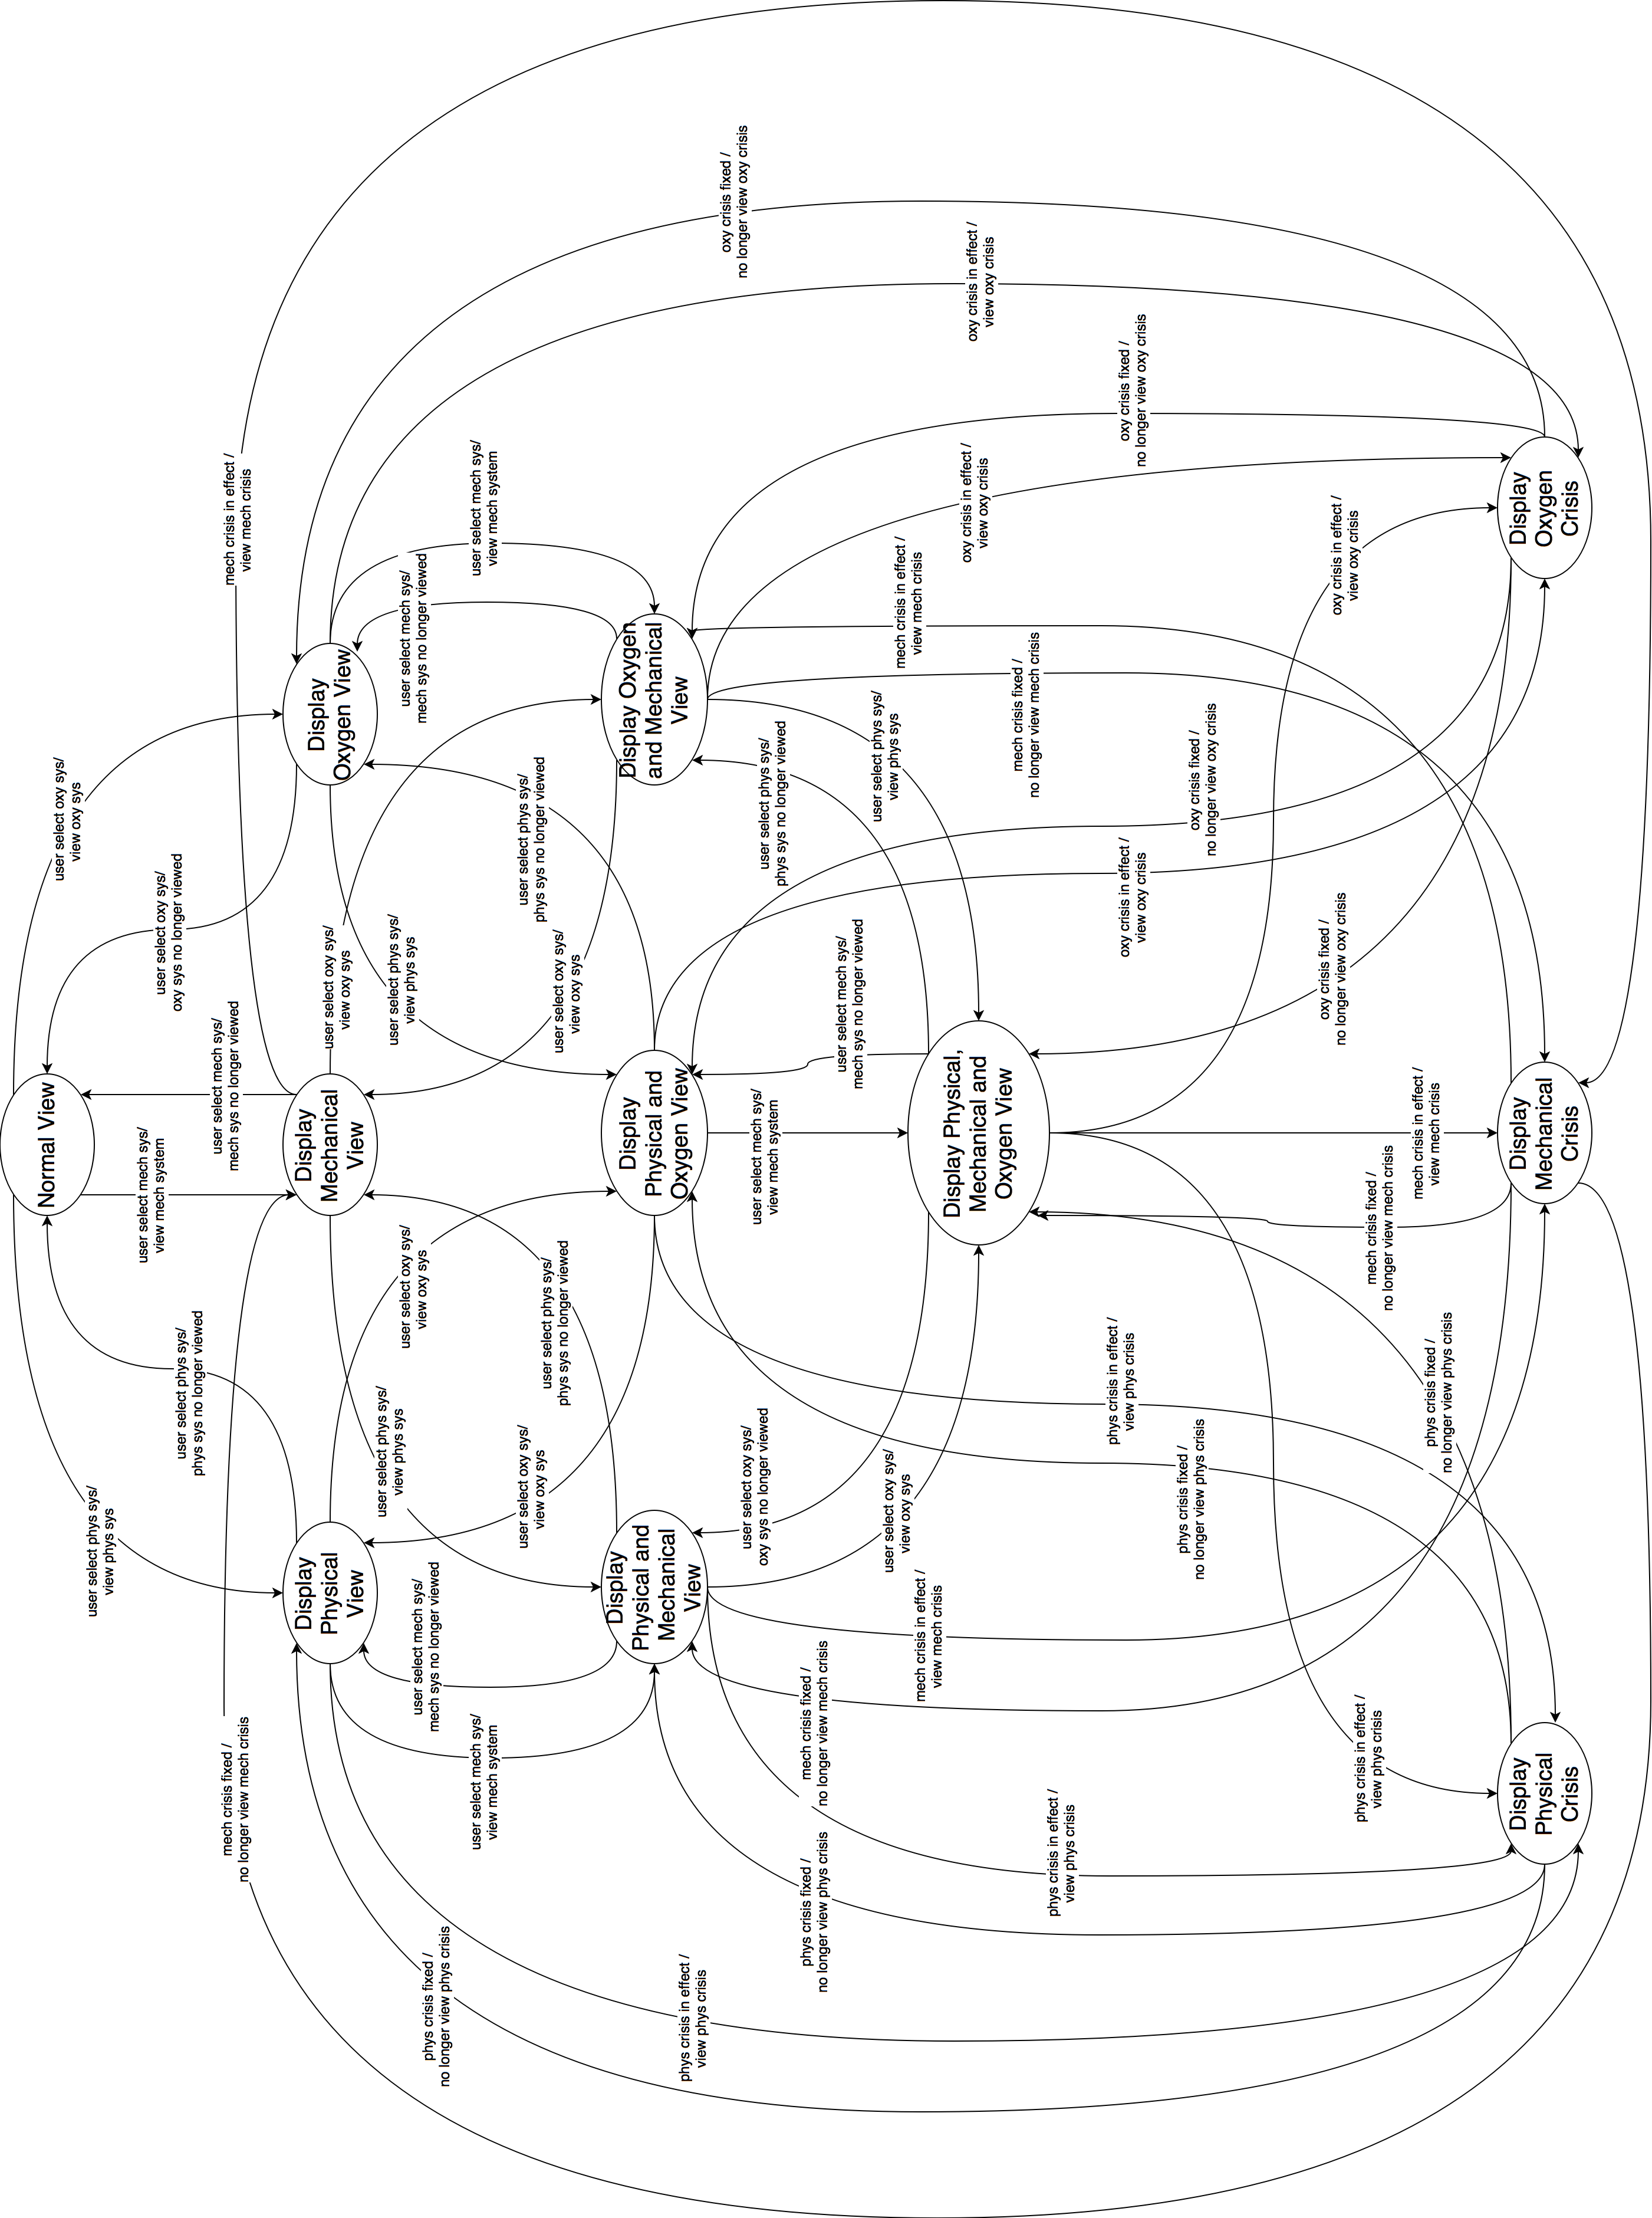
\includegraphics[width=180mm]{OC.png}
\caption{Oxygen Controller State Chart}
\end{figure}
% End Section

\section{Sequence Diagrams}
\label{sec:sequence_diagrams}
\subsection*{Start Simulation}
\begin{figure}[H]
\centering
\includegraphics[scale = 0.5]{"Start Simulation".jpg}
\caption{Start Simulation Sequence Diagram}
\end{figure}
\subsection*{End Simulation}
\begin{figure}[H]
\centering
\includegraphics[scale = 0.5]{"Stop Simulation".jpg}
\caption{End Simulation Sequence Diagram}
\end{figure}
\subsection*{Pause Simulation}
\begin{figure}[H]
\centering
\includegraphics[scale = 0.5]{"Pause Simulation".jpg}
\caption{Pause Simulation Sequence Diagram}
\end{figure}
\subsection*{Resume Simulation}
\begin{figure}[H]
\centering
\includegraphics[scale = 0.5]{"Resume Simulation".jpg}
\caption{Resume Simulation Sequence Diagram}
\end{figure}
\subsection*{View Overall Simulation}
\begin{figure}[H]
\centering
\includegraphics[scale = 0.35]{"Overall View".jpg}
\caption{Overall View Sequence Diagram}
\end{figure}
\subsection*{View Power System}
\begin{figure}[H]
\centering
\includegraphics[scale = 0.5]{"View Power System".jpg}
\caption{View Power System Sequence Diagram}
\end{figure}
\subsection*{View Oxygen System}
\begin{figure}[H]
\centering
\includegraphics[scale = 0.5]{"View Oxygen System".jpg}
\caption{View Oxygen System Sequence Diagram}
\end{figure}
\subsection*{View Mechanical System}
\begin{figure}[H]
\centering
\includegraphics[scale = 0.5]{"View Mechanical System".jpg}
\caption{View Mechanical System Sequence Diagram}
\end{figure}
\subsection*{Fix Crisis}
\begin{figure}[H]
\centering
\includegraphics[scale = 0.5]{"Untitled Diagram (3)".png}
\caption{Fix Crisis Sequence Diagram}
\end{figure}
\subsection*{Fix Power}
\begin{figure}[H]
\centering
\includegraphics[scale = 0.5]{"Untitled Diagram".png}
\caption{Fix Power Sequence Diagram}
\end{figure}
\subsection*{Fix Oxygen}
\begin{figure}[H]
\centering
\includegraphics[scale = 0.5]{"Untitled Diagram (2)".png}
\caption{Fix Oxygen Sequence Diagram}
\end{figure}
\subsection*{Fix Mechanical}
\begin{figure}[H]
\centering
\includegraphics[scale = 0.5]{"Untitled Diagram (1)".png}
\caption{Fix Mechanical Sequence Diagram}
\end{figure}

\section{Detailed Class Diagram}
\label{sec:detailed_class_diagram}
\begin{figure}[H]
\centering
\includegraphics[width=180mm]{"Class Diagram".png}
\caption{Detailed Class Diagram}
\end{figure}
\newpage
\appendix
\section{Division of Labour}
\label{sec:division_of_labour}
% Begin Section
\begin{table}[h!]
\centering


\begin{tabular}{|c|c|c|}
\hline
{\bf Member} & {\bf Duties}&{\bf Signature}\\
\hline
{David Hobson} & {Detailed Class Diagram} & { }\\
{} & {Editing}  & {}\\
\hline
{Pavle Arezina} & {Introduction} & {}\\
{} & {Sequence Diagrams} & {}\\
{} & {Editing} & {}\\
\hline
{Pareek Ravi} & {Sequence Diagrams} & {}\\
{} & {} & {}\\
\hline
{Victoria Graff} & {State Chart Diagrams} & {}\\
{} & {} & {}\\
\hline
{Julian Cassano} & {Detailed Class Diagram} & {}\\
{} & {} & {}\\
\hline
\end{tabular}

\end{table}
% End Section




\end{document}
%------------------------------------------------------------------------------